\documentclass[17pt, t, lualatex]{beamer}

\title{Understanding Kelvin-Helmholtz Instabilities}
\date{May 27, 2025}
\institute[KTH]{KTH Royal Institute of Technology}
\author{Paul Mayer}

\usepackage{amsmath,amssymb,mathtools}
\usepackage{multicol}

% Probably load as late as possible
% Other options are
% - engine=pdflatex to compile in pdfLaTeX (with different fonts),
% - mathshape=rm to use serif font for math,
% - mathsahpe=custom to not set any math font (so that you can define your own math fonts)
\usetheme[engine=lualatex, mathshape=sf, fontdir=kthpq-files/fonts/Figtree/]{kthpq}
\setmonofont{Bitstream Vera Sans Mono}[Scale=.9]

% Custom colors (see beamercolorthemecustom.sty for more details)
%\usecolortheme{custom}

% Modify the headline template: KTH-full, KTH-section-only, or KTH-frametitle-only.
%\setbeamertemplate{headline}[KTH-full]

% Custom footline
%\setfootline{left}{center}{right}

\begin{document}

\inserttitlepage

\section{Introduction}
%\insertsectionpage

\begin{frame}{Kelvin-Helmholtz Instabilities}
\begin{columns}
\begin{column}{0.5\textwidth}
\begin{center}
    \begin{figure}
        \centering
        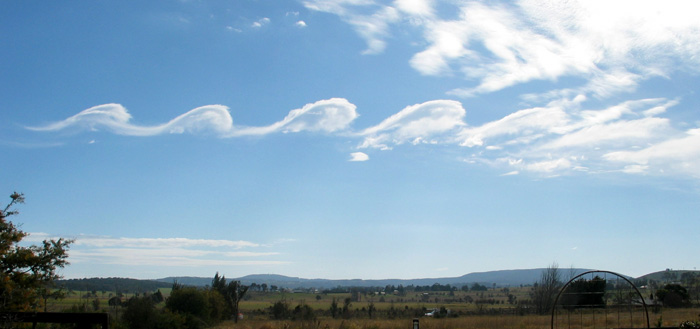
\includegraphics[width=1\linewidth]{imgs/clouds}
        \caption{Clouds forming characteristic vortices.}
        \label{fig:clouds}
    \end{figure}
\end{center}
\end{column}
\begin{column}{0.5\textwidth}
\begin{center}
    \begin{figure}
        \centering
        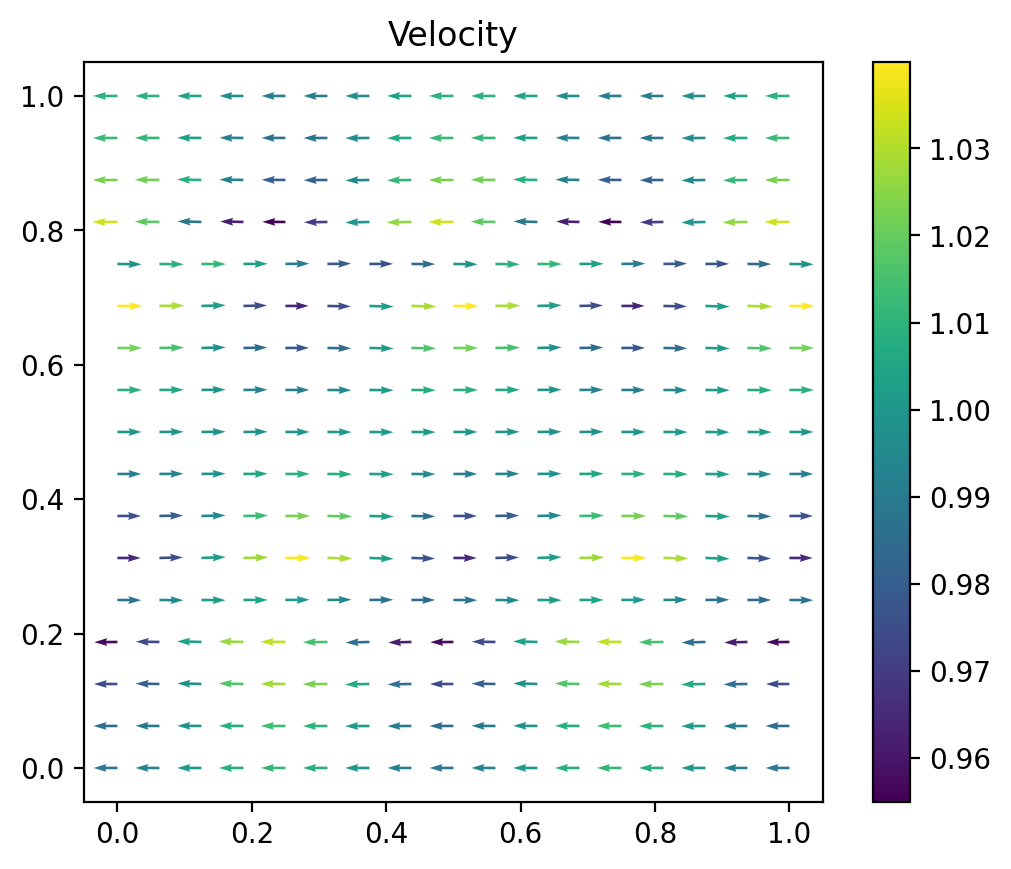
\includegraphics[width=.7\linewidth]{imgs/shear}
        \caption{Velocity shear induces instabilities.}
        \label{fig:shear}
    \end{figure}
\end{center}
\end{column}
\end{columns}
\end{frame}

\section{Methodology}
%\insertsectionpage

\begin{frame}{Setup}
\begin{columns}
\begin{column}{0.5\textwidth}
   \begin{block}{Incompressible Navier-Stokes Eqns}
   \begin{align*}
       \frac{\partial u}{\partial t} + (u\cdot \nabla)u + \nabla p -\Delta u &= 0,\\\nabla \cdot u &= 0.
   \end{align*}
    In weak form:
    \begin{align*}
       (\dot u + (u\cdot \nabla)u, v) - (p,\nabla \cdot v) + (\nu \nabla u,\nabla v) &+ \\
       (\nabla \cdot u, q) + SD(u,p;v,q&) = (f,v)
    \end{align*}
    \end{block}
\end{column}
\begin{column}{0.5\textwidth}
    \begin{block}{Boundary Conditions}
    \begin{itemize}
        \item $x = 0, x = 1$:\\
        Periodic boundary conditions
        \item $y = 0, y = 1$:\\
        Free-slip boundary conditions
    \end{itemize}
    \end{block}
    \begin{block}{Initial Conditions}
        $v = \begin{pmatrix}-1 + 2 * (\text{abs}(x[1] - 0.5) <= 0.5)\\
        \psi(x,y)\end{pmatrix}$\\
        $p = 2.5$
    \end{block}
\end{column}
\end{columns}
\end{frame}

\begin{frame}{Questions}
\begin{itemize}
    \item How sensitive is the simulation on grid resolution?
    \item How does the Reynolds Number change the behaviour of the instability?
\end{itemize}
\end{frame}

\section{Demo}
\insertsectionpage
\section{Future Work}
\begin{frame}{Measure vortex intensity}
\begin{figure}
    \centering
    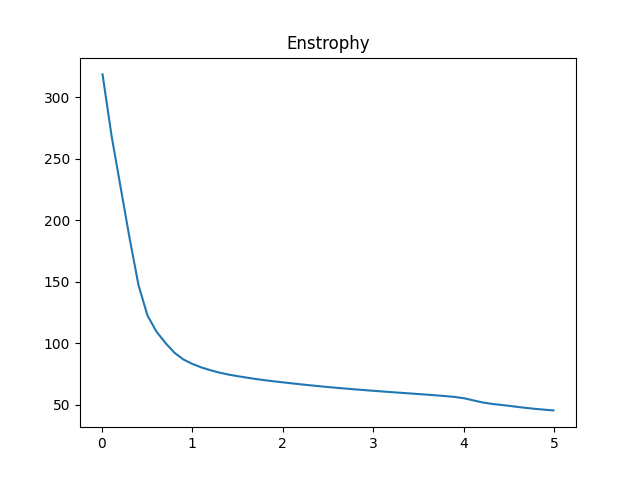
\includegraphics[width=.5\linewidth]{imgs/enstrophy}
    \caption{Integral of curl field.}
    \label{fig:enstrophy}
\end{figure}
\end{frame}

\begin{frame}{Measure vortex intensity}
\begin{figure}
    \centering
    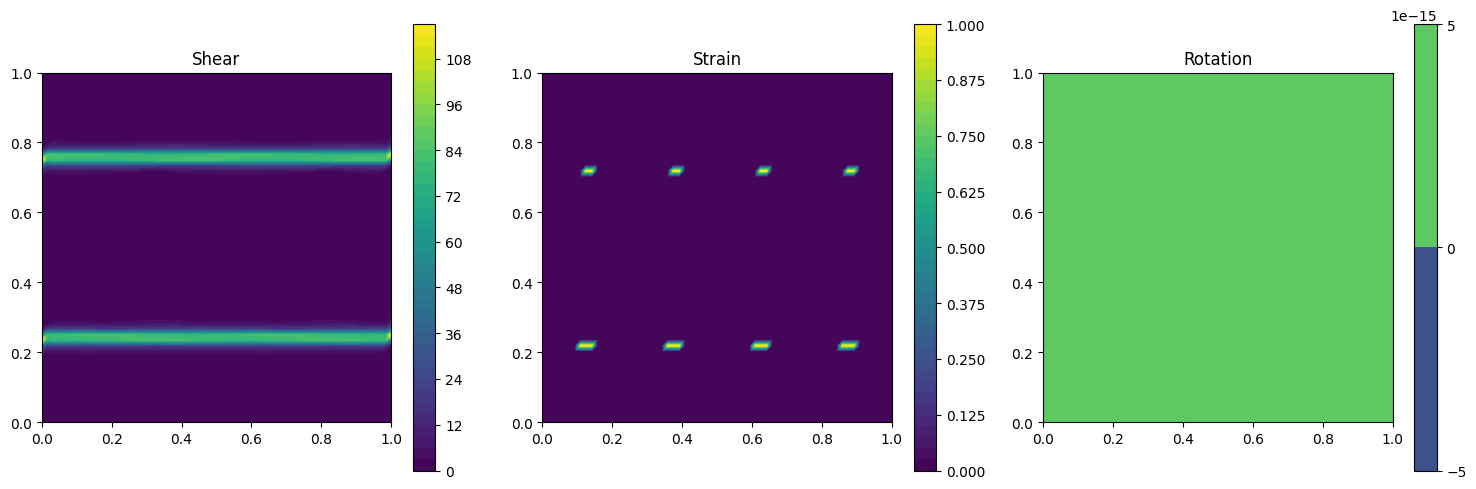
\includegraphics[width=1\linewidth]{imgs/rotation1}
    \caption{Triple decomposition t=0}
    \label{fig:triple_decomp1}
\end{figure}
\end{frame}
\begin{frame}{Measure vortex intensity}
\begin{figure}
    \centering
    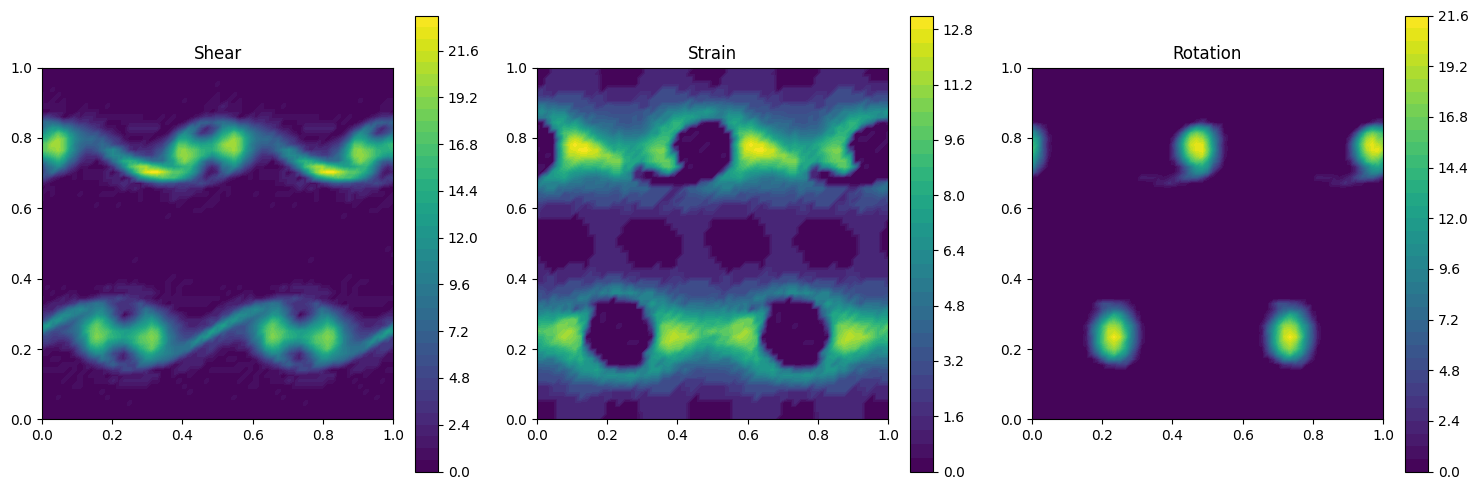
\includegraphics[width=1\linewidth]{imgs/rotation2}
    \caption{Triple decomposition t=1}
    \label{fig:triple_decomp2}
\end{figure}
\end{frame}
\insertendpage

\section{Appendix}
\insertsectionpage
\begin{frame}{Appendix A}
\end{frame}

\end{document}